\documentclass[11pt]{article}
\usepackage[a4paper,bindingoffset=0.2in,%
left=1in,right=1in,top=0.5in,bottom=0.3in,%
footskip=.15in]{geometry}
\usepackage[T1]{fontenc}
\usepackage{titling}
\usepackage{interval}
\usepackage{scalerel}
\usepackage{amsmath}
\usepackage{graphicx}
\usepackage{subcaption}

\author{Artur Pyśk \\ Aleksander Szewczak \\ grupa 2 - Aplikacje internetowe i bazy danych}
\title{%
  Algorytmy numeryczne - zadanie 2 \\
  \large Operacje na macierzach}
\date{18 listopada 2018r.}

\begin{document}
 \maketitle
Sprawozdanie pokazuje analizę poprawnościową oraz wydajnościową algorytmu eliminacji Gaussa w następujących wariantach:
\begin{description}
  \item[G:] bez wyboru elementu podstawowego
  \item[PG:] z częściowym wyborem elementu podstawowego
  \item[FG:] z pełnym wyborem elementu podstawoewgo
\end{description}
Testy zostały przeprowadzone na komputerze Lenovo IdeaPad 510-15ISK wyposażonym w procesor Intel Core i5-6200 (2,4 GHz), pamięć 8GB RAM DDR3 i system Windows 10. Testując algorytm używalimy następujących typów reprezentujących liczbę rzeczywistą:
\begin{description}
  \item[TF:] typ pojedynczej precyzji: float
  \item[TD:] typ podwójnej precyzji: double
  \item[TC:] typ własny: Fraction
\end{description}
Program, który napisaliśmy w języku C\scalerel*{\#}{X} rozwiązuje układ równań $A \cdot X = B$ dla losowej macierzy kwadratowej $A$ i wektora $B$. Jako współczynniki macierzy $A$ i wektora $X$ wzięliśmy pseudolosowe liczby zmiennoprzecinkowe z przedziału [-1,1) otrzymane jako iloraz $\frac{x}{2^{16}}$, gdzie $x$ jest pseudolosową liczbą całkowitą z przedziału [$-2^{16}$,$2^{16}-1$]. Wektor $B$ obliczamy jako $B:=A \cdot X$. Macierz $A$ i wektor $B$ podajemy jako parametry do rozwiązania układu równań, wektor $X$ zachowujemy jako rozwiązanie wzorcowe. 
\\[1\baselineskip]
Aby udowodnić, że algorytm Gaussa został zaimplementowany poprawnie, porównaliśmy wyniki naszego programu dla typu float wraz z wynikami obliczonymi przez WolframAlpha dla macierzy o rozmiarze 2x2.
\\[1\baselineskip]
Macierz $A = $
$\begin{bmatrix}
    -0.006820267871      & 0.958740234  \\
    -0.7615204       & 0.996871948
\end{bmatrix}$
, Wektor $B = $
$\begin{bmatrix}
   0.763859749  \\
   0.603664458
\end{bmatrix}$
\\[1\baselineskip]
Zestawienie wyników:
\\[1\baselineskip]
\begin{tabular}{cccc}
Wolfram & G & PG & FG \\
$\begin{bmatrix}
    0.573548  \\
    0.0200814
\end{bmatrix}$ 
& 
$\begin{bmatrix}
    0.573547363  \\
    0.0200805664
\end{bmatrix}$ 
& 
$\begin{bmatrix}
    0.5735474  \\
    0.0200805664
\end{bmatrix}$ 
& 
$\begin{bmatrix}
    0.5735474  \\
   0.0200814
\end{bmatrix}$
\end{tabular}
\\[1\baselineskip]
Jak można zauważyć, wyniki są niemal identyczne, natomiast powstaje niewielki błąd, który jest spowodowany nieprecyzyjnością typu zmiennoprzecinkowego.
\newpage
\section{Hipotezy}
H1: Dla dowolnego ustalonego rozmiaru macierzy czas działania metody Gaussa w kolejnych
wersjach (1, 2, 3) rośnie.

\begin{figure}[h!]
  \centering
  \begin{subfigure}[b]{0.45\linewidth}
    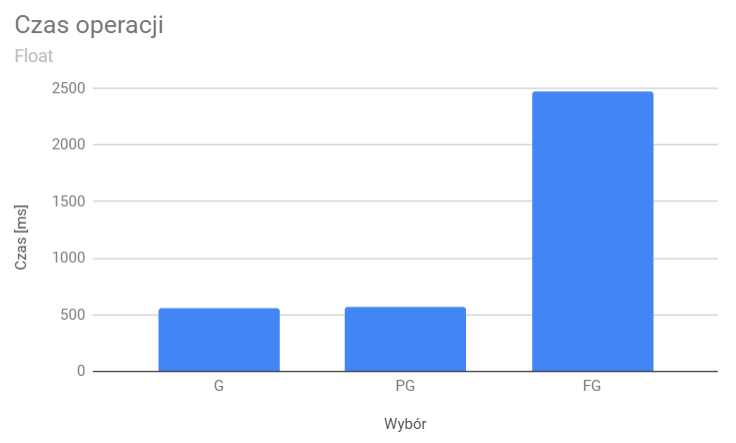
\includegraphics[width=\linewidth]{wykres_czas_float.png}
    \caption{Float ($N = 500$)}
  \end{subfigure}
  \begin{subfigure}[b]{0.45\linewidth}
    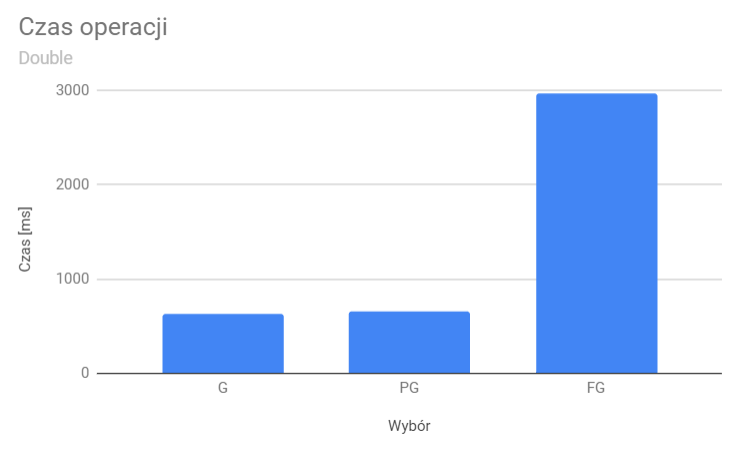
\includegraphics[width=\linewidth]{wykres_czas_double.png}
    \caption{Double ($N = 500$)}
  \end{subfigure}
\begin{subfigure}[b]{0.45\linewidth}
    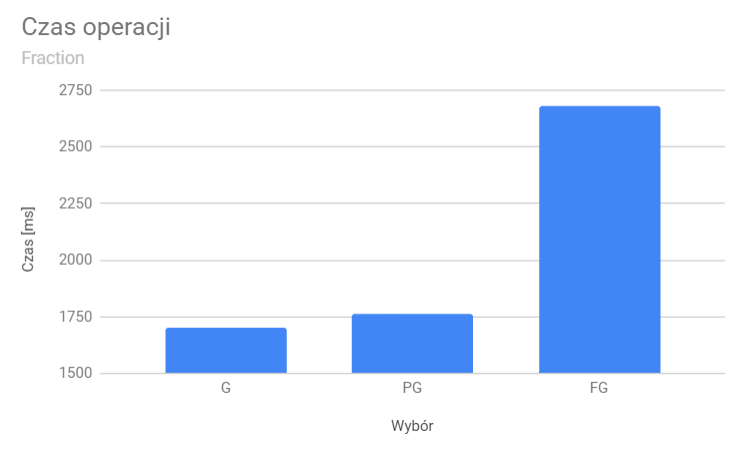
\includegraphics[width=\linewidth]{wykres_czas_fraction.png}
    \caption{Fraction ($N = 50$)}
  \end{subfigure}
  \label{fig:wykres}
\end{figure}

Jak możemy zauważyć na powyższych wykresach, zarówno dla typu Float jak i Double, dla $N = 500$ oraz typu Fraction, dla $N = 50$, czas działania metody Gaussa w kolejnych wersjach (1 ,2, 3) rośnie. Przy kilkunastu próbach dostrzegliśmy, że nie ma dużej różnicy miedzy wariantami G i PG. Co jest zastanawiające, w kilku przypadkach czas wariantu PG jest mniejszy niż G. Prawdopodobine jest to spowodowane tym, że w kilku testach PG został uruchomiony później niż G. Wariant FG jest zdecydowanie najwolniejszy. Okazuje się, że hipoteza jest prawdziwa dla większości przypadków. W zależności od ustalonego $N$ algorytm PG wykonuje się nieznacznie dłużej niż G. Wariant FG zawsze trwa największą ilość czasu.
\\[1\baselineskip]
H2: Dla dowolnego ustalonego rozmiaru macierzy błąd uzyskanego wyniku metody
Gaussa w kolejnych wersjach (1, 2, 3) maleje.

\begin{figure}[h!]
  \centering
  \begin{subfigure}[b]{0.45\linewidth}
    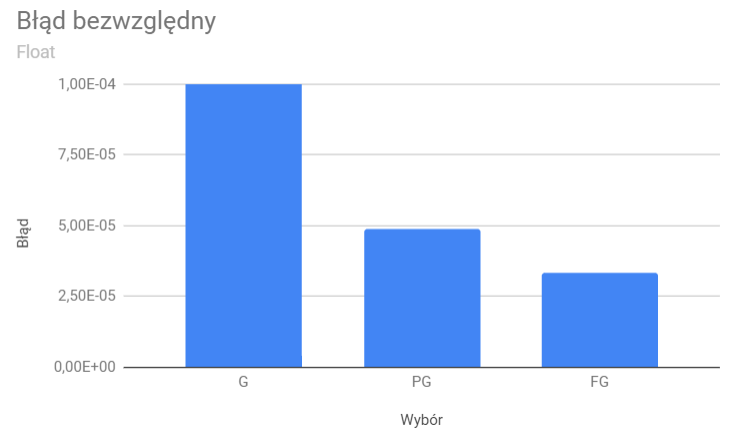
\includegraphics[width=\linewidth]{wykres_blad_float.png}
    \caption{Float}
  \end{subfigure}
  \begin{subfigure}[b]{0.45\linewidth}
    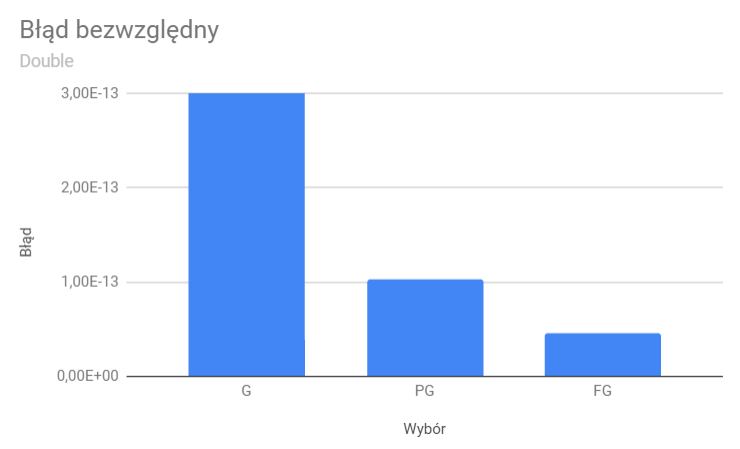
\includegraphics[width=\linewidth]{wykres_blad_double.png}
    \caption{Double}
  \end{subfigure}
  \label{fig:wykres}
\end{figure}

Jak zauważamy na powyższym wykresie, zarówno dla typu Float jak i Double, dla $N = 500$, błąd uzyskanego wyniku metody Gaussa w kolejnych wersjach (1, 2, 3) maleje. W przypadku obu typów, największy błąd następuje przy wariancie G. Błędy wariantów PG i FG są sobie bliższe, natomiast największą dokładność ma algorytm z pełnym wyborem. Okazuje się, że hipoteza jest prawdziwa dla wszystkich przypadków. Najbardziej korzystny jednak wydaje się algorytm Gaussa z częściowym wyborem biorąc pod uwagę stosunek jego dokładności do wydajności. Wykonuje się sporo krócej, niż wariant FG, natomiast daje zbliżone wyniki. Dla własnego typu Fraction, błąd dla każdego wariantu jest taki sam - równy $0$. Dlaczego tak się dzieje, wyjaśniamy w poniższej hipotezie.
\\[1\baselineskip]
H3: Użycie własnej arytmetyki na ułamkach zapewnia bezbłędne wyniki niezależnie od
wariantu metody Gaussa i rozmiaru macierzy.
\begin{center}
 \begin{tabular}{|c | c| c | c|c|c|c|} 
 \hline
 n & B(G) & B(PG) & B(FG) & T(G) & T(PG) & T(FG)  \\ 
 \hline\hline
 10 & 0 & 0 & 0 & 23 & 24 & 29 \\ 
 \hline
 20 & 0 & 0 & 0 & 309 & 321 & 491 \\
 \hline
 30 & 0 & 0 & 0 & 1293 & 1353 & 1705 \\
 \hline
 40 & 0 & 0 & 0 & 4298 & 4613 & 5698 \\
 \hline
 50 & 0 & 0 & 0 & 10865 & 11492 & 14840 \\ 
 \hline
\end{tabular}
\end{center}
Patrząc na powyższą tabelę prezentującą własny typ Fraction, gdzie B - błąd bezwzględny, T - czas [ms] dochodzimy do wniosku, że użycie własnej arytmetyki eliminuje błąd obliczeń. Dzięki wykorzystaniu typu BigInteger, który nie posiada żadnego limitu przechowywania danych (jedynym ograniczeniem jest nasz komputer) możemy wykonywać skomplikowane obliczenia bez błędów. Hipoteza jest więc prawdziwa. Użycie własnej arytmetyki na ułamkach zapewnia bezbłędne wyniki niezależnie od wariantu metody Gaussa i rozmiaru macierzy. Z powodu ograniczeń sprzętowych, ciężko było nam zrobić odpowiednie testy dla większych macierzy.
\section{Pytania}
Q1: Jak zależy dokładność obliczeń (błąd) od rozmiaru macierzy dla dwóch wybranych
przez Ciebie wariantów metody Gaussa gdy obliczenia prowadzone są na typie
podwójnej precyzji (TD)?
\begin{figure}[h!]
  \centering
  \begin{subfigure}[b]{0.45\linewidth}
    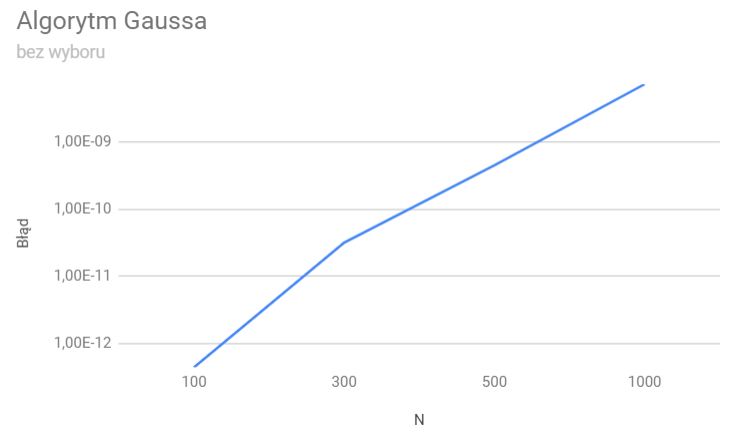
\includegraphics[width=\linewidth]{wykres_blad_g_double.png}
    \caption{Bez wyboru}
  \end{subfigure}
  \begin{subfigure}[b]{0.45\linewidth}
    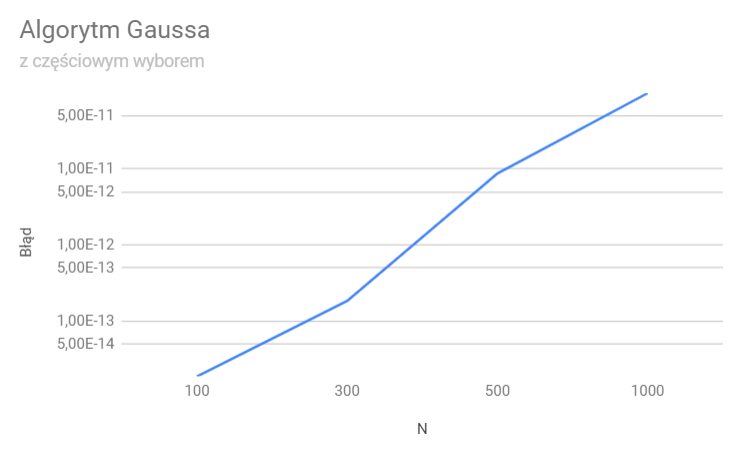
\includegraphics[width=\linewidth]{wykres_blad_pg_double.png}
    \caption{Z częściowym wyborem}
  \end{subfigure}
  \label{fig:wykres}
\end{figure}
\\[1\baselineskip]
Do testów, które umożliwiły nam odpowiedź na to pytanie skorzystaliśmy z wariantów G oraz PG. Jak możemy zauważyć na powyższym wykresie, im większa macierz, tym błąd rośnie i wynik staje się mniej dokładny. Dokładność obliczeń maleje wraz z wzrostem rozmiaru macierzy.
\\[1\baselineskip]
Q2: Jak przy wybranym przez Ciebie wariancie metody Gaussa zależy czas działania
algorytmu od rozmiaru macierzy i różnych typów?
\begin{figure}[h!]
  \centering
  \begin{subfigure}[b]{0.8\linewidth}
    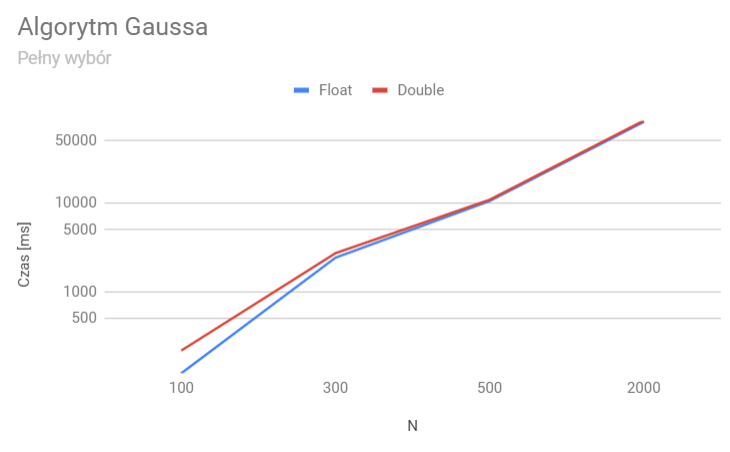
\includegraphics[width=\linewidth]{wykres_czasy_fg.png}
  \end{subfigure}
  \label{fig:wykres}
\end{figure}
\\[1\baselineskip]
Do testów, które umożliwiły nam odpowiedź na to pytanie skorzystaliśmy z wariantu FG. Jak możemy zauważyć na poniższym wykresie oraz tabeli z hipotezy trzeciej, im większa macierz tym dłuższy czas wykonywania algorytmu, niezależnie od typu. Typ double wykonuje się trochę dłużej niż typ float. Najdłuższy czas działania ma jednak własny typ Fraction.
\newpage
\section{Wydajność implementacji}
\begin{center}
 \begin{tabular}{|c | c| c | c|} 
\hline
 Typ & T(G) & T(PG) & T(FG)  \\ 
 \hline
\multicolumn{4}{ |c| }{n = 500} \\
\hline
 Float & 554ms & 569ms & 2473ms \\ 
 \hline
 Double & 633ms & 651ms & 2966ms \\
 \hline
\multicolumn{4}{ |c| }{n = 100} \\
 \hline
 Fraction & 246179ms & 247009ms & 322440ms \\
 \hline
\end{tabular}
\end{center}
Z powodu ograniczeń komputera, testowanie typu z własną arytmetyką ograniczyliśmy do macierzy dla N = 100.
Zdecydowanie najdłużej wykonuje się typ własnej arytmetyki. Typ double wykonuje się trochę dłużej niż float, ale nie ma ogromnej różnicy.
\section{Podział pracy}
\begin{center}
 \begin{tabular}{|c | c|} 
 \hline
 Aleksander Szewczak & Artur Pyśk  \\ 
 \hline\hline
 Praca nad strukturą projektu & Praca nad strukturą projektu  \\ 
 \hline
 Algorytm - warianty PG i FG & Algorytm - wariant G  \\
 \hline
 Przeprowadzenie testów & Implementacja klasy generycznej MyMatrix  \\
 \hline
 Generowanie wykresów & Implementacja typu własnej precyzji Fraction \\
 \hline
 Przygotowanie sprawozdania & Obliczanie błędu  \\ 
 \hline
\end{tabular}
\end{center}
\end{document}